\chapter{Technical Analysis}\label{ch:solutionProposal}
This chapter will propose different types of sensors, wheel systems, energy sources, general materials and software.

\section{Sensors}
For a robot to scan its surrounding area for mapping and obstacle avoidance, it requires sensors to do so.

\subsection{Radar}
Radars use a highly concentrated radio wave, if there are any obstacles in its way, they will reflect electromagnetic energy. The sensor will then pick up the signalling energy and measure the time spent on receiving the echo\cite{Radar}.
The further away the transmission has to be sent, the lower the frequency has to be.\\
Satellites are typically using C-band ( 300 MHz - 1 GHz ). 
For avoidance on the other hand, it will be of higher frequencies, since the system has to maneuver at high accuracy. This frequency for avoidance will be generalized at I- or J-band (8-12 GHz)\cite{RadarTutorial}.

%\begin{figure}[h]
    %\centering
   % 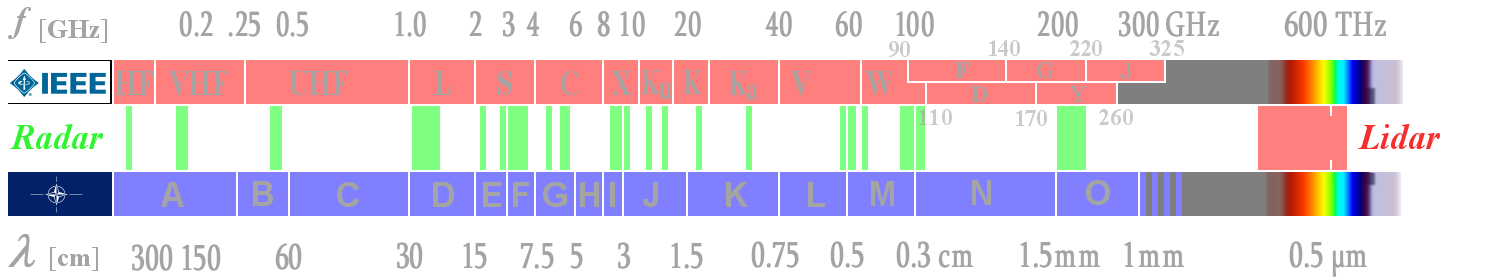
\includegraphics[width=\textwidth]{figures/radarfrequencies.png}
  %  \caption{Radar Frequencies \cite{RadarTutorial}}
 %   \label{fig:radarfrequencies.png}
%\end{figure}


\subsection{LIDAR}\label{ch:sensorLidar}
LIDAR offers a wide variety of hardware to implement. Many of these cameras have a high spinning rate and offers a precise cloud of 3D data. These precise readings will help the robot to measure accurate distances towards objects. This will give the robot more maneuverability and make the remote control more manageable when the pictures received are clear. The 3D data cloud will also help the robot to move autonomously.\\
A good example is the Velodyne HDL-64, which can collect 1.3 million 3D points per second, and has a rotation rate of 10.4 HZ. With a 360${^\circ}$ field of vision and looking up to 120 meter into the distance, this would be a very effecient hardware implementation. \cite{Lidar360}

\subsection{Cameras (RGB-D)} \label{ch:CameraRGB}
A RGB-D camera gives a color image and provides a depth per pixel. This project will use an RGB-D.
The RGB-D has a color camera and is based on PrimeSense patent.  
PrimeSense uses a sensor that projects an infrared speckle pattern and an IR camera will then capture the pattern. This is called structured light. This light will project a triangular image for the image sensor processor to process. It will then derive the range and bearing for the illuminated object from the beam of structured light and match it to the current position of the vehicle\cite{Lasers}.\\
Comparing each point collected and the stored pattern in the RGB-D camera, which is calibrated to a known depth, the RGB-D camera produces an image with depth information for each pixel\cite{RGB-D-new}.
%A downside to the IR cameras is that it does not work well in sunlight. This is because the infrared light rays interferes with the IR camera\cite{IR}.

\subsection{Ultrasonic sensors}
Ultrasonic sensors use sound waves to measure distance to various obstacles. One part of the sensor called a transducer, emits a sound wave that hits the surface, bounces back and gets picked up by the receiver. 
%To calculate how far away a set of objects is, the wave formula is needed to calculate the velocity of the wave. Lambda is the wavelength, f is the frequency of the wave and v is the velocity.
%\begin{equation}\label{eq:ultrasonic01}
 %   v= \lambda \cdot f
%\end{equation}
%For calculating distance(d) back and forwards the velocity is needed and the time (t) for the signal to be sent and received. 
%\begin{equation}\label{eq:unltrasonic02}
 %  d=t\cdot v 
%\end{equation}
%The distance has to be halved, because the time is from the transducer to the receiver.
%\begin{equation}\label{eq:unltrasonic03}
 %  DTO=d/2
%\end{equation}
Ultrasonic sensors sounds can deflect different from some surfaces, which is a problem. They can also be sensitive to noise in the signal and the sensor does not have a good sense of direction. This can be overcome by using an array of ultrasonic sensors to help build up a more accurate map, by having multiple inputs from the array\cite{Ultrasonicsnesor}.
%\newpage

